%═══════════════════════════════════════════════════════════════════════════════
\section{Nondeterministic Turing Machines (slides 30--45)} \kemark
%═══════════════════════════════════════════════════════════════════════════════

This is the second major extension to the basic TM model, and arguably the most
important one in all of theoretical computer science. Multi-tape machines
(Section~4) made machines \emph{faster}. Nondeterministic machines make them
\emph{easier to design} --- and they are the foundation of the P vs.\ NP
question you'll meet in Lectures 6--7.

We take our time here. By the end of this section you will be able to:
\begin{enumerate}[nosep]
\item Explain nondeterminism in plain English and distinguish it from randomness.
\item Write the formal definition of an NTM and explain every symbol.
\item Draw computation trees and determine acceptance from them.
\item Construct NTMs using the ``guess and verify'' pattern.
\item Prove that every NTM can be simulated by a DTM (the simulation theorem).
\end{enumerate}

%───────────────────────────────────────────────────────────────────────────────
\subsection{What Is Nondeterminism? (slides 30--31)}
\label{subsec:what-is-nondeterminism}
%───────────────────────────────────────────────────────────────────────────────

\begin{notebox}{Analogy --- The Maze with Self-Cloning}
Imagine you're standing at the entrance of a giant hedge maze. There's a prize
at the exit. You have two possible strategies:

\textbf{Strategy 1 (deterministic):} Pick one rule, like ``always turn left,''
and follow it. You explore exactly one path. If that path hits a dead end, you
backtrack and try another. You walk one step at a time, following \emph{one}
trail of footprints. This might take forever if the maze is huge --- you could
wander down a very long dead end before ever finding the exit.

\textbf{Strategy 2 (nondeterministic):} Every time you reach a fork, you
\textbf{clone yourself}. One clone takes the left path, another takes the
right path, a third takes the middle path --- as many clones as there are
options. Each clone continues independently. If it hits another fork, it clones
again. You now have an \emph{army} of copies exploring \emph{every possible
path simultaneously}. The moment \textbf{any single clone} finds the exit, you
declare: ``I solved the maze!''

The nondeterministic solver doesn't randomly guess --- it explores
\textbf{all possibilities at once}. One success is enough.

\textbf{In our formal world:}
\begin{itemize}[nosep]
\item Maze = the computation on input $w$
\item Fork in the maze = a configuration where $|\delta(q, a)| > 1$
  (the transition function offers multiple choices)
\item Clone = a branch in the computation tree
\item Exit (the prize) = an accepting configuration (reaching state $t$)
\item ``I solved the maze!'' = the NTM accepts
\item One path through the maze = one computation (one root-to-leaf path in the tree)
\end{itemize}
\end{notebox}

\begin{conceptbox}{Nondeterminism $\neq$ Randomness --- This Distinction Is Critical}
\textbf{The mistake almost everyone makes:} ``Nondeterministic just means the
machine picks randomly, right?'' \textbf{No. Absolutely not.}

Here is the difference, made concrete:

\begin{center}
\renewcommand{\arraystretch}{1.4}
\begin{tabular}{p{4cm}p{5.5cm}p{5.5cm}}
\toprule
& \textbf{Randomized (probabilistic)} & \textbf{Nondeterministic} \\
\midrule
\textbf{At a fork} & Flip a coin and take ONE path &
  Clone and take ALL paths simultaneously \\
\textbf{Number of paths explored} & Exactly one (chosen by chance) &
  All of them (every possible path) \\
\textbf{Can it be wrong?} & Yes --- the coin might choose a bad path &
  Never --- if a good path \emph{exists}, some clone finds it \\
\textbf{Acceptance} & Accept with some \emph{probability} &
  Accept if \emph{any} path reaches $t$ \\
\textbf{Real-world analog} & Rolling dice to navigate the maze &
  Cloning at every fork \\
\bottomrule
\end{tabular}
\end{center}

\textbf{Example to feel the difference.} Suppose a maze has 1,000 paths, and
exactly 1 leads to the exit.
\begin{itemize}[nosep]
\item \textbf{Randomized:} picks one path at random. Probability of success:
  $1/1000 = 0.1\%$. Might fail!
\item \textbf{Nondeterministic:} explores all 1,000 paths simultaneously. One
  clone finds the exit. \textbf{Always succeeds.}
\end{itemize}

\kt{Nondeterminism is not ``guessing randomly.'' It is ``trying every possibility
at once and succeeding if any one of them works.'' Random picks ONE path;
nondeterministic explores ALL paths.}
\end{conceptbox}

\begin{conceptbox}{Why We Care About Nondeterminism}
Three reasons nondeterminism matters in this course:

\begin{enumerate}
\item \textbf{Machine design becomes dramatically easier.} For some languages,
  the deterministic TM needs a complicated state machine to track partial
  matches. The nondeterministic TM just ``guesses'' where the interesting thing
  happens and checks. You'll see this with our running example: ``contains 110.''

\item \textbf{NP is defined using NTMs.} In Lectures 6--7, you'll learn that
  $\text{NP}$ = the set of languages decidable by a \emph{nondeterministic}
  Turing machine in polynomial time. Understanding NTMs is a prerequisite
  for understanding P vs.\ NP, arguably the biggest open question in computer
  science.

\item \textbf{NTMs don't add power --- and that's surprising.} Despite the
  ``magical'' ability to explore all paths at once, an NTM can't solve any
  problem that a DTM can't. A DTM can simulate any NTM by systematically trying
  all branches (Section~5.10). The simulation is slower, but it always works.
  Same story as multi-tape: more convenience, not more power.
\end{enumerate}

\kt{Nondeterminism makes machines easier to design, is the foundation of the
complexity class NP, and --- surprisingly --- does NOT add computational power
over deterministic TMs.}
\end{conceptbox}

%───────────────────────────────────────────────────────────────────────────────
\subsection{NFA Reminder --- Nondeterminism in Finite Automata (from Semester 1)}
\label{subsec:nfa-reminder}
%───────────────────────────────────────────────────────────────────────────────

Before we define NTMs, let's recall the simpler version of nondeterminism you
already saw in Semester 1: nondeterministic finite automata (NFAs). This is the
same idea, just for a weaker machine model.

\begin{notebox}{Quick Recall: DFA vs.\ NFA}
A \textbf{DFA} has a transition function $\delta \colon Q \times \Sigma \to Q$
--- for each state and input symbol, there is exactly \textbf{one} next state.
No choice.

An \textbf{NFA} has a transition function
$\delta \colon Q \times \Sigma \to 2^Q$ --- for each state and input symbol,
there is a \textbf{set} of possible next states. The machine can ``go to''
\emph{any} of them simultaneously.

\textbf{NFA acceptance:} the NFA accepts $w$ if there \textbf{exists} at least
one path through the states that ends in an accepting state. Most paths might
die or reject --- doesn't matter. One accepting path is enough.

\textbf{The Semester 1 punchline:} NFAs and DFAs recognize exactly the same
class of languages (the \emph{regular} languages). NFAs are more convenient for
design, but they can't recognize any language that a DFA can't. The proof:
the subset construction simulates an NFA with a DFA.

\textbf{The Lecture 2 parallel:} NTMs and DTMs recognize exactly the same class
of languages (the \emph{computably-enumerable} languages). NTMs are more
convenient, but they can't solve any problem that a DTM can't. The proof:
the BFS simulation (Section~5.10). \textbf{Same idea, bigger machine.}
\end{notebox}

\begin{examplebox}{{NFA Example: Strings Containing 10001}}

This NFA ``guesses'' where the substring \texttt{10001} starts and then
verifies the next five characters match. Before the guess, it stays in the
start state reading anything. After successful verification, it stays in the
accepting state reading anything.

\begin{center}
\begin{tikzpicture}[node distance=2cm, on grid, >=Stealth,
    every state/.style={thick, fill=blue!5, minimum size=0.9cm}]
    % States
    \node[state, initial]                (q0) {$q_0$};
    \node[state, right=of q0]           (q1) {$q_1$};
    \node[state, right=of q1]           (q2) {$q_2$};
    \node[state, right=of q2]           (q3) {$q_3$};
    \node[state, right=of q3]           (q4) {$q_4$};
    \node[state, accepting, right=of q4](q5) {$q_5$};

    % Transitions
    \path[->]
      (q0) edge [loop above] node {$0,1$} ()
      (q0) edge              node [above] {$1$}   (q1)
      (q1) edge              node [above] {$0$}   (q2)
      (q2) edge              node [above] {$0$}   (q3)
      (q3) edge              node [above] {$0$}   (q4)
      (q4) edge              node [above] {$1$}   (q5)
      (q5) edge [loop above] node {$0,1$} ();
\end{tikzpicture}
\end{center}

\textbf{How to read this diagram:}
\begin{itemize}[nosep]
\item $q_0$ is the start state (arrow from nowhere). It has a self-loop on both
  $0$ and $1$ --- meaning it can stay in $q_0$ reading anything, waiting to
  ``guess'' that the substring starts now.
\item At any point while in $q_0$ and reading a $1$, the NFA can
  \textbf{nondeterministically} choose to either stay in $q_0$ (via the
  self-loop) \textbf{or} move to $q_1$ (beginning verification).
\item From $q_1$, the path is deterministic: must read $0$, then $0$, then $0$,
  then $1$, matching the substring $10001$.
\item $q_5$ is the accepting state (double circle) with a self-loop --- once
  you've verified the substring, you accept regardless of what comes after.
\item If the NFA guesses wrong (e.g., moves to $q_1$ but the next character
  isn't $0$), that branch ``dies'' --- there's no transition, so it gets stuck.
  But other branches (the ones that stayed in $q_0$) continue.
\end{itemize}

\kt{NFA acceptance = there EXISTS a path from start to accept. The NTM will work
the same way, but with a tape instead of just states.}
\end{examplebox}

%───────────────────────────────────────────────────────────────────────────────
\subsection{NTM Formal Definition (slides 32--33)}
\label{subsec:ntm-formal-def}
%───────────────────────────────────────────────────────────────────────────────

\begin{notebox}{Analogy --- GPS Showing All Routes}
Imagine a GPS navigation app. A normal GPS picks the ``best'' route and shows
you \textbf{one} path from A to B. That's deterministic --- one input (your
location and destination), one output (a single route).

Now imagine a magical GPS that shows you \textbf{every possible route}
simultaneously --- every combination of streets, highways, and shortcuts, all
overlaid on the map at once. You can see all of them. If \emph{any single route}
reaches the destination, the GPS says ``route found!''

This magical GPS is a nondeterministic Turing machine. At every intersection
(configuration with multiple transition options), it takes \emph{all} possible
turns. Each route is a branch. If any branch reaches the destination (state
$t$), the machine accepts.

\textbf{In our formal world:}
\begin{itemize}[nosep]
\item GPS app = the NTM $M$
\item Your location = the current configuration $\gamma$
\item Intersection with multiple options = a configuration where
  $|\delta(q, a)| > 1$
\item Each route on the map = one branch of the computation tree
\item Destination reached = the branch reaches state $t$
\item ``Route found!'' = the NTM accepts
\end{itemize}
\end{notebox}

\begin{definitionbox}{Nondeterministic Turing Machine (NTM)}

\textbf{Plain English:}
A nondeterministic Turing machine is exactly like a deterministic Turing
machine, except for one change: when the machine is in some state $q$ reading
some symbol $a$, instead of having exactly one thing it \emph{must} do, it has
a \textbf{set} of things it \emph{could} do. It ``does all of them at once''
(conceptually). If any one of those parallel computations reaches the accept
state, the machine accepts.

\textbf{Formal Definition:}

An NTM is a 7-tuple:
\fitmath{M = (Q,\; \Sigma,\; \Gamma,\; s,\; t,\; r,\; \delta)}

where all components are the same as a DTM, \textbf{except} the transition
function:

\fitmath{\delta \colon (Q \setminus \{t, r\}) \times \Gamma \;\to\; 2^{Q \times \Gamma \times \{-1, +1\}}}

\textbf{Breaking Down the Notation:}
\begin{itemize}[nosep]
\item $Q$ = finite set of states (same as DTM)
\item $\Sigma$ = input alphabet (same as DTM)
\item $\Gamma$ = tape alphabet with $\Sigma \cup \{\sqcup\} \subseteq \Gamma$
  (same as DTM)
\item $s \in Q$ = start state (same as DTM)
\item $t \in Q$ = accept state (same as DTM)
\item $r \in Q$ = reject state, $r \neq t$ (same as DTM)
\item $\delta$ = the transition function --- \textbf{this is the ONLY difference}:
  \begin{itemize}[nosep]
  \item \textbf{Domain:} $(Q \setminus \{t, r\}) \times \Gamma$ --- same as DTM.
    In non-halting state $q$, reading tape symbol $a$.
  \item \textbf{Codomain:} $2^{Q \times \Gamma \times \{-1, +1\}}$ --- the
    \textbf{power set} of $Q \times \Gamma \times \{-1, +1\}$.
  \item $2^S$ means ``the set of all subsets of $S$.'' So $\delta(q, a)$ returns
    a \textbf{set} of (state, symbol, direction) triples, not just one triple.
  \end{itemize}
\end{itemize}

\textbf{What this means concretely.} Suppose:
\fitmath{\delta(q, a) = \{(q_1, b_1, +1),\; (q_2, b_2, -1)\}}

Then from the configuration where the machine is in state $q$ reading $a$,
there are \textbf{two} possible next configurations:
\begin{enumerate}[nosep]
\item Go to state $q_1$, write $b_1$, move right.
\item Go to state $q_2$, write $b_2$, move left.
\end{enumerate}
The NTM ``takes both'' --- it branches into two parallel computations.

If $\delta(q, a) = \{(q_1, b_1, +1)\}$ (a set with one element), then there is
no choice --- exactly one next configuration. This is the deterministic case.

\kt{A DTM is a special case of an NTM where $|\delta(q,a)| = 1$ for every
$(q,a)$ pair. Every DTM is already an NTM that just never branches.}
\end{definitionbox}

\begin{examplebox}{DTM vs.\ NTM --- Side-by-Side Comparison}
\begin{center}
\renewcommand{\arraystretch}{1.5}
\begin{tabular}{p{3.5cm}p{5.5cm}p{5.5cm}}
\toprule
& \textbf{DTM} & \textbf{NTM} \\
\midrule
\textbf{Transition function} &
  $\delta \colon (Q \setminus \{t,r\}) \times \Gamma \to Q \times \Gamma \times \{-1,+1\}$ &
  $\delta \colon (Q \setminus \{t,r\}) \times \Gamma \to 2^{Q \times \Gamma \times \{-1,+1\}}$ \\
\textbf{Returns} &
  Exactly one triple $(q', b, d)$ &
  A set of triples $\{(q_1, b_1, d_1), \ldots\}$ \\
\textbf{Successor configs} &
  Exactly 1 &
  0, 1, 2, 3, \ldots\ (could be many) \\
\textbf{Computation shape} &
  A \textbf{line} (sequence of configs) &
  A \textbf{tree} (branching at nondeterministic steps) \\
\textbf{Acceptance} &
  The single computation reaches $t$ &
  $\exists$ at least one branch reaching $t$ \\
\textbf{Rejection} &
  The single computation reaches $r$ or loops forever &
  ALL branches reach $r$ or loop (none reaches $t$) \\
\bottomrule
\end{tabular}
\end{center}

\kt{The ONLY difference between a DTM and an NTM is that $\delta$ returns a set
instead of a single element. Everything else --- states, tape, alphabet ---
is identical.}
\end{examplebox}

%───────────────────────────────────────────────────────────────────────────────
\subsection{The Computation Tree (slides 34--35)}
\label{subsec:computation-tree}
%───────────────────────────────────────────────────────────────────────────────

\begin{notebox}{Analogy --- Choose Your Own Adventure Book}
Remember ``Choose Your Own Adventure'' books? You start on page 1. At the
bottom of each page, you make a choice: ``If you open the door, turn to
page 47. If you climb the window, turn to page 23. If you run away, turn to
page 89.''

Each choice leads to a different storyline. Some storylines end with ``You
Win!'' (accepting). Some end with ``You Lose!'' (rejecting). Some go on
forever because you're stuck in a loop of pages that keep pointing to each
other (infinite loop).

A deterministic reader follows \textbf{one} storyline. A nondeterministic
reader follows \textbf{all} storylines simultaneously. If \emph{any} storyline
says ``You Win!'' --- you win.

The full collection of all possible storylines, organized by which choices
lead where, forms a \textbf{tree}. That's the computation tree.

\textbf{In our formal world:}
\begin{itemize}[nosep]
\item Page 1 = the initial configuration $\alpha_w$ (state $s$, input $w$ on
  tape, head at position 0)
\item A choice at the bottom of a page = a nondeterministic branch where
  $|\delta(q, a)| > 1$
\item Each storyline = one root-to-leaf path in the computation tree
\item ``You Win!'' ending = a leaf node in state $t$ (accept)
\item ``You Lose!'' ending = a leaf node in state $r$ (reject)
\item Infinite story (stuck in a loop) = an infinite branch (no leaf)
\end{itemize}
\end{notebox}

\begin{definitionbox}{Computation Tree of an NTM}

\textbf{Plain English:}
The computation tree is a picture of \emph{everything} that can happen when an
NTM $M$ runs on input $w$. The root is the starting configuration. Each node is
a configuration. The children of a node are all the configurations that the NTM
could transition to from that node (one child per element of $\delta(q, a)$).

\textbf{Formal Definition:}
Given NTM $M$ and input $w$, the \textbf{computation tree} $T_M(w)$ is:
\begin{itemize}[nosep]
\item \textbf{Root:} the initial configuration $\alpha_w$
\item \textbf{Children of node $\gamma$:} for configuration $\gamma$ in state
  $q$ reading symbol $a$, the children are all configurations reachable via one
  step --- one child for each $(q', b, d) \in \delta(q, a)$
\item \textbf{Leaves:} configurations in state $t$ (accept) or state $r$
  (reject) --- these have no children because $\delta$ is undefined for $t$
  and $r$
\item \textbf{Infinite branches:} if a path never reaches $t$ or $r$, it
  continues forever (the branch has no leaf)
\end{itemize}

\textbf{Key properties:}
\begin{enumerate}[nosep]
\item The tree may be \textbf{infinite} --- either because branches are infinite
  (loops) or because the branching creates an infinite number of nodes.
\item The \textbf{branching factor} at any node is bounded by $|\delta(q, a)|$
  --- the number of options in the transition set. If the maximum over all
  $(q, a)$ pairs is $b$, then each node has at most $b$ children.
\item \textbf{Branches are independent.} What happens on one branch has
  absolutely no effect on any other branch. Each branch is its own separate
  computation with its own copy of the tape.
\end{enumerate}
\end{definitionbox}

Now let's draw a \textbf{concrete} computation tree. We'll use the NTM for
``contains 110'' (which we'll construct in detail in Section~5.8) running on
input \texttt{0110}. For now, here is the key idea: the machine scans left to
right, and at every $1$ it reads, it can either (a)~keep scanning or (b)~start
verifying that ``110'' appears starting here. Option (b) commits it to checking
the next two symbols.

\begin{examplebox}{Computation Tree: NTM for ``contains 110'' on input 0110}

The NTM has states $\{s, q_1, q_{11}, t, r\}$. We show the full tree. Each
node shows (state, tape, head position). Tape positions are 0-indexed;
$\sqcup$ is blank. We underline the character under the head.

\textbf{Level 0 (root):}

The initial configuration. State $s$, tape = $0110\sqcup$, head at position 0.

\textbf{Level 1:}

In state $s$ reading $0$: $\delta(s, 0) = \{(s, 0, +1)\}$. Only one option: stay in $s$, move right. \textbf{No branching.}

\textbf{Level 2:}

Now in state $s$ at position 1, reading $1$: $\delta(s, 1) = \{(s, 1, +1),\;
(q_1, 1, +1)\}$. \textbf{Two options --- the tree branches!}

\textbf{Levels 3--4:} Each branch continues until it hits $t$ or $r$.

Here is the full tree:

\begin{center}
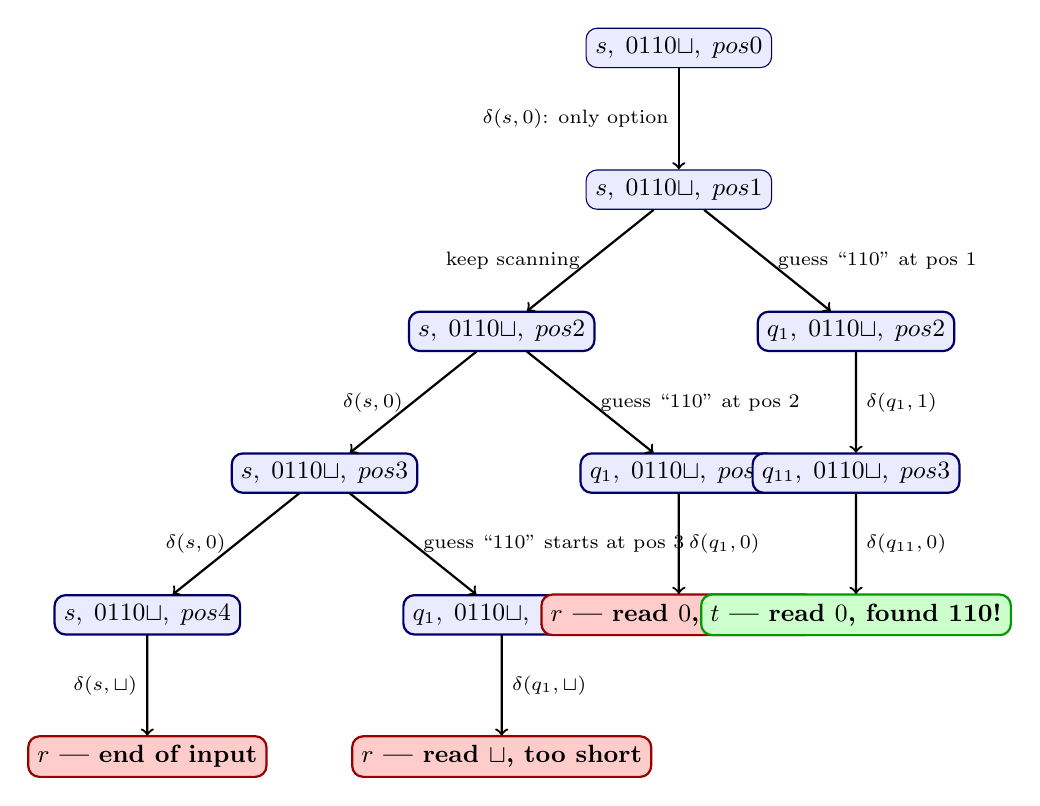
\begin{tikzpicture}[
    level distance=1.8cm,
    sibling distance=4.5cm,
    edge from parent/.style={draw, ->, thick},
    every node/.style={font=\small},
    acc/.style={fill=green!20, draw=green!60!black, rounded corners, font=\small\bfseries},
    rej/.style={fill=red!20, draw=red!60!black, rounded corners, font=\small\bfseries},
    cfg/.style={fill=blue!8, draw=blue!40!black, rounded corners, font=\small},
  ]
  \node[cfg] {$s,\; 0110\sqcup,\; \text{pos } 0$}
    child {
      node[cfg] {$s,\; 0110\sqcup,\; \text{pos } 1$}
        child {
          node[cfg] {$s,\; 0110\sqcup,\; \text{pos } 2$}
            child {
              node[cfg] {$s,\; 0110\sqcup,\; \text{pos } 3$}
                child {
                  node[cfg] {$s,\; 0110\sqcup,\; \text{pos } 4$}
                    child {
                      node[rej] {$r$ --- end of input}
                      edge from parent node[left, font=\scriptsize] {$\delta(s, \sqcup)$}
                    }
                  edge from parent node[left, font=\scriptsize] {$\delta(s, 0)$}
                }
                child {
                  node[cfg] {$q_1,\; 0110\sqcup,\; \text{pos } 4$}
                    child {
                      node[rej] {$r$ --- read $\sqcup$, too short}
                      edge from parent node[right, font=\scriptsize] {$\delta(q_1, \sqcup)$}
                    }
                  edge from parent node[right, font=\scriptsize] {guess ``110'' starts at pos 3}
                }
              edge from parent node[left, font=\scriptsize] {$\delta(s, 0)$}
            }
            child {
              node[cfg] {$q_1,\; 0110\sqcup,\; \text{pos } 3$}
                child {
                  node[rej] {$r$ --- read $0$, not ``1''}
                  edge from parent node[right, font=\scriptsize] {$\delta(q_1, 0)$}
                }
              edge from parent node[right, font=\scriptsize] {guess ``110'' at pos 2}
            }
          edge from parent node[left, font=\scriptsize] {keep scanning}
        }
        child {
          node[cfg] {$q_1,\; 0110\sqcup,\; \text{pos } 2$}
            child {
              node[cfg] {$q_{11},\; 0110\sqcup,\; \text{pos } 3$}
                child {
                  node[acc] {$t$ --- read $0$, found 110!}
                  edge from parent node[right, font=\scriptsize] {$\delta(q_{11}, 0)$}
                }
              edge from parent node[right, font=\scriptsize] {$\delta(q_1, 1)$}
            }
          edge from parent node[right, font=\scriptsize] {guess ``110'' at pos 1}
        }
      edge from parent node[left, font=\scriptsize] {$\delta(s, 0)$: only option}
    };
\end{tikzpicture}
\end{center}

\textbf{Reading the tree:}
\begin{itemize}[nosep]
\item The root is the initial configuration. The machine reads $0$ in state $s$
  --- only one option, so no branching at level 0$\to$1.
\item At position 1, the machine reads $1$ in state $s$. \textbf{Two options:}
  keep scanning (stay in $s$) or guess that ``110'' starts here (go to $q_1$).
  The tree branches.
\item \textbf{Right branch} (guess at position 1): moves to $q_1$, reads $1$ at
  position 2 (good --- second ``1'' found, go to $q_{11}$), reads $0$ at
  position 3 (good --- found ``110''!). \textbf{Reaches state $t$.}
  \textcolor{green!60!black}{\textbf{ACCEPT.}}
\item \textbf{Left branch} continues scanning. At position 2, reads $1$ ---
  branches again. At position 3, reads $0$ --- branches again. Various
  sub-branches try to verify ``110'' starting at positions 2 and 3, but those
  guesses are wrong (position 2: next char is $0$, not $1$; position 3: next
  char is $\sqcup$, too short). They all reach $r$.
\item The leftmost branch scans all the way to the blank and rejects.
\end{itemize}

\textbf{Result:} At least one branch (the right branch from position 1) reaches
$t$. Therefore, the NTM \textbf{accepts} $0110$.

\kt{The computation tree for NTM on $0110$ has one accepting leaf (green) and
several rejecting leaves (red). Since at least one path reaches $t$, the NTM
accepts. This is the ``exists'' rule in action.}
\end{examplebox}

%───────────────────────────────────────────────────────────────────────────────
\subsection{NTM Acceptance: The ``Exists'' Rule (slides 36--37)}
\label{subsec:ntm-acceptance}
%───────────────────────────────────────────────────────────────────────────────

\begin{notebox}{Analogy --- University Applications}
You apply to 10 universities. You get accepted by 3, rejected by 5, and
2 never respond (they ``loop'' forever in their admissions process). The
question: \textbf{are you accepted to university?}

\textbf{YES.} You got into 3 schools. That's enough. The 5 rejections and the
2 non-responses don't cancel out the 3 acceptances. You're going to university.
One acceptance is all you need.

\textbf{In our formal world:}
\begin{itemize}[nosep]
\item 10 universities = 10 branches of the NTM's computation tree
\item 3 accepted = 3 branches reach state $t$
\item 5 rejected = 5 branches reach state $r$
\item 2 never respond = 2 branches loop forever (infinite branches)
\item ``You're accepted!'' = the NTM accepts $w$
\end{itemize}

Now consider a different scenario: you apply to 10 universities. 7 reject you,
3 never respond. \textbf{Are you accepted?} NO --- no one said yes. The fact
that 3 are still ``thinking'' doesn't help. You don't have an acceptance letter.
\end{notebox}

\begin{definitionbox}{NTM Acceptance and Language Recognition}

\textbf{Plain English:}
An NTM accepts a word $w$ if there is \emph{at least one} way the computation
can reach the accept state $t$. It doesn't matter if other branches reject or
loop forever. One success is enough.

\textbf{Formal Definition:}
\begin{itemize}[nosep]
\item $M$ \textbf{accepts} $w$ if $\exists$ a computation of $M$ on $w$ that
  halts in state $t$.
\item $M$ \textbf{does not accept} $w$ if no computation of $M$ on $w$ halts
  in $t$.
  (Every branch either reaches $r$ or loops forever.)
\item The \textbf{language recognized by $M$}:
  \fitmath{L(M) = \{w \in \Sigma^* \mid M \text{ accepts } w\} = \{w \in \Sigma^* \mid \exists \text{ computation of } M \text{ on } w \text{ halting in } t\}}
\end{itemize}

\textbf{Breaking Down the Key Points:}
\begin{itemize}[nosep]
\item \textbf{``$\exists$ a computation''} --- existential quantifier. Not ``for
  all,'' not ``most,'' not ``with high probability'' --- just \textbf{at least
  one}.
\item \textbf{``Does not accept'' is NOT the same as ``rejects.''} An NTM does
  not accept $w$ if no branch reaches $t$. This could be because all branches
  reach $r$ (reject), OR because some branches loop forever and the rest reach
  $r$. Either way: no branch hits $t$, so the word is not accepted.
\item \textbf{Accepts vs.\ rejects vs.\ loops:} Consider an NTM on input $w$:
  \begin{itemize}[nosep]
  \item If some branch reaches $t$ $\Rightarrow$ \textbf{accepts} (regardless
    of other branches)
  \item If all branches reach $r$ $\Rightarrow$ \textbf{rejects}
  \item If no branch reaches $t$, but some branches loop $\Rightarrow$
    \textbf{does not accept} (and we can't definitively say ``reject'' because
    the machine doesn't halt on all branches)
  \end{itemize}
\end{itemize}

\kt{NTM acceptance = $\exists$ (there exists) a branch reaching $t$.
NTM non-acceptance = $\forall$ (for all) branches, none reaches $t$.}
\end{definitionbox}

To make this concrete, let's look at all the possible scenarios:

\begin{examplebox}{All Possible Scenarios for NTM on Input $w$}

Imagine an NTM with 4 branches on some input $w$. Here are all the interesting
combinations:

\begin{center}
\renewcommand{\arraystretch}{1.4}
\begin{tabular}{cccccc}
\toprule
\textbf{Scenario} & \textbf{Branch 1} & \textbf{Branch 2} & \textbf{Branch 3}
& \textbf{Branch 4} & \textbf{NTM result} \\
\midrule
A & $t$ & $r$ & $r$ & $r$ & \textbf{Accepts} \\
B & $t$ & $t$ & $r$ & loops & \textbf{Accepts} \\
C & $t$ & $t$ & $t$ & $t$ & \textbf{Accepts} \\
D & $r$ & $r$ & $r$ & $r$ & \textbf{Does not accept} \\
E & $r$ & $r$ & loops & loops & \textbf{Does not accept} \\
F & loops & loops & loops & loops & \textbf{Does not accept} \\
\bottomrule
\end{tabular}
\end{center}

\textbf{Key observations:}
\begin{itemize}[nosep]
\item Scenarios A, B, C: at least one branch reaches $t$ $\Rightarrow$ accepts.
  It doesn't matter that other branches reject or loop.
\item Scenario D: all branches reject $\Rightarrow$ does not accept (and we can
  also say the machine ``rejects,'' since every branch halted in $r$).
\item Scenario E: some reject, some loop $\Rightarrow$ does not accept. But
  the machine doesn't cleanly ``reject'' either, because it hasn't halted on
  all branches. It just\ldots\ never finishes, partially.
\item Scenario F: all branches loop $\Rightarrow$ does not accept.
\end{itemize}
\end{examplebox}

%───────────────────────────────────────────────────────────────────────────────
\subsection{Exercise 3: The Five Wrong Definitions (slides 37--38)}
\label{subsec:five-wrong-defs}
%───────────────────────────────────────────────────────────────────────────────

The lecture presents five candidate definitions for ``$M$ accepts $w$'' and asks
which are correct. This is a classic exam-style question that tests whether you
\emph{really} understand the ``$\exists$'' in NTM acceptance.

\begin{conceptbox}{Exercise 3 --- Five Candidate Definitions for NTM Acceptance}
Consider an NTM $M$ and input $w$. Which of the following correctly defines
``$M$ accepts $w$''?

\begin{center}
\renewcommand{\arraystretch}{1.6}
\begin{tabular}{clcc}
\toprule
\textbf{\#} & \textbf{Statement} & \textbf{Verdict} & \textbf{Correct?} \\
\midrule
1 & More than one computation halts in $t$ & WRONG & \textcolor{red!70!black}{$\boldsymbol{\times}$} \\
2 & No computation halts in $r$ & WRONG & \textcolor{red!70!black}{$\boldsymbol{\times}$} \\
3 & There exists a computation halting in $t$ & RIGHT & \textcolor{green!60!black}{$\boldsymbol{\checkmark}$} \\
4 & Exactly one accepting computation & WRONG & \textcolor{red!70!black}{$\boldsymbol{\times}$} \\
5 & Every computation halts in $t$ & WRONG & \textcolor{red!70!black}{$\boldsymbol{\times}$} \\
\bottomrule
\end{tabular}
\end{center}

Now let's understand \textbf{exactly why} each wrong answer is wrong, with
concrete counterexamples.
\end{conceptbox}

\begin{examplebox}{Why Statement 1 Is Wrong: ``More Than One Computation Halts in $t$''}

\textbf{The statement:} ``$M$ accepts $w$ if more than one computation halts in
$t$.'' This requires $\geq 2$ accepting branches.

\textbf{Why it's wrong:} One accepting branch is enough. The actual definition
only requires $\exists$ (at least one), not $\geq 2$.

\textbf{Counterexample:} Consider an NTM with 5 branches. Exactly 1 reaches
$t$, the other 4 reach $r$.

By the \textbf{real definition}: $M$ accepts $w$ (there exists a computation
halting in $t$ --- namely branch 1).

By \textbf{statement 1}: $M$ does NOT accept $w$ (only one computation halts in
$t$, not ``more than one'').

Statement 1 is \textbf{too strong} --- it demands multiple successes when one is
enough.
\end{examplebox}

\begin{examplebox}{Why Statement 2 Is Wrong: ``No Computation Halts in $r$''}

\textbf{The statement:} ``$M$ accepts $w$ if no computation halts in $r$.''

\textbf{Why it's wrong:} This confuses the \emph{absence of rejection} with
\emph{acceptance}. What if no branch reaches $t$ AND no branch reaches $r$?
That happens when all branches loop forever.

\textbf{Counterexample:} Consider an NTM where \textbf{all} branches loop
forever on input $w$. No branch reaches $t$, no branch reaches $r$.

By the \textbf{real definition}: $M$ does NOT accept $w$ (no computation halts
in $t$).

By \textbf{statement 2}: $M$ accepts $w$ (``no computation halts in $r$'' is
true, since no computation halts at all!).

Statement 2 would incorrectly say looping = accepting. The real definition says
looping = not accepting.
\end{examplebox}

\begin{examplebox}{Why Statement 3 Is Right: ``There Exists a Computation Halting in $t$''}

\textbf{The statement:} ``$M$ accepts $w$ if there exists a computation halting
in $t$.''

\textbf{This IS the definition.} The word ``exists'' ($\exists$) is doing all
the work. At least one branch reaching $t$ is necessary and sufficient.
\begin{itemize}[nosep]
\item If 1 out of 1000 branches reaches $t$: accepts.
\item If 999 out of 1000 branches reach $t$: accepts.
\item If 0 out of 1000 branches reach $t$: does not accept.
\end{itemize}
\end{examplebox}

\begin{examplebox}{Why Statement 4 Is Wrong: ``Exactly One Accepting Computation''}

\textbf{The statement:} ``$M$ accepts $w$ if exactly one computation halts in
$t$.''

\textbf{Why it's wrong:} Having multiple accepting branches is perfectly fine.
The definition says ``at least one,'' not ``exactly one.''

\textbf{Counterexample:} Consider an NTM where \textbf{3} branches reach $t$
and 2 branches reach $r$ on input $w$.

By the \textbf{real definition}: $M$ accepts $w$ (there exists a computation
halting in $t$ --- in fact, three of them).

By \textbf{statement 4}: $M$ does NOT accept $w$ (three computations halt in
$t$, not ``exactly one'').

Statement 4 is wrong in the opposite direction of statement 1 --- it insists on
\emph{exactly} one success, when any positive number of successes should count.
\end{examplebox}

\begin{examplebox}{Why Statement 5 Is Wrong: ``Every Computation Halts in $t$''}

\textbf{The statement:} ``$M$ accepts $w$ if every computation halts in $t$.''

\textbf{Why it's wrong:} This replaces $\exists$ (there exists) with $\forall$
(for all). It requires \emph{unanimous} acceptance --- every branch must accept.
The real definition only needs one.

\textbf{Counterexample:} Consider our ``contains 110'' NTM on input $0110$.
We saw in Section~5.4 that one branch reaches $t$ but several branches reach
$r$ (the ``wrong guesses'').

By the \textbf{real definition}: $M$ accepts $0110$ (there exists a computation
halting in $t$).

By \textbf{statement 5}: $M$ does NOT accept $0110$ (not every computation halts
in $t$ --- most branches reject!).

Statement 5 is \textbf{far too strong}. If we required every branch to accept,
nondeterminism would be useless --- the machine would only accept inputs where
\emph{every} guess works, which defeats the whole purpose of branching.

\kt{The correct definition uses $\exists$ (at least one branch accepts).
Statement 5 uses $\forall$ (all branches must accept). These are completely
different quantifiers, and confusing them is the \#1 mistake with NTMs.}
\end{examplebox}

%───────────────────────────────────────────────────────────────────────────────
\subsection{Halting NTM (slide 39)}
\label{subsec:halting-ntm}
%───────────────────────────────────────────────────────────────────────────────

\begin{notebox}{Analogy --- Adventure Book Where Every Story Ends}
Remember the ``Choose Your Own Adventure'' analogy? Some adventure books are
well-written: every storyline eventually reaches an ending --- either ``You
Win!'' or ``You Lose!'' There are no circular page references that trap you in
an infinite loop.

A \textbf{halting NTM} is like a well-written adventure book: every branch of
the computation tree eventually reaches either $t$ (accept) or $r$ (reject).
No branch goes on forever. The tree is \textbf{finite}.

\textbf{In our formal world:}
\begin{itemize}[nosep]
\item Well-written book = halting NTM
\item Every story ends = every branch of the computation tree is finite
\item No infinite loops = no infinite branches in the tree
\item The whole tree is finite = the computation tree has finitely many nodes
\end{itemize}
\end{notebox}

\begin{definitionbox}{Halting NTM}

\textbf{Plain English:}
A halting NTM is an NTM that always terminates, no matter what input you give
it and no matter which branch you follow. Every single branch of the computation
tree reaches either the accept state $t$ or the reject state $r$ in finitely
many steps.

\textbf{Formal Definition:}
An NTM $M$ is \textbf{halting} if for every input $w \in \Sigma^*$, the
computation tree $T_M(w)$ is \textbf{finite} --- i.e., every branch has finite
length (every branch terminates in $t$ or $r$).

\textbf{Consequence for acceptance:}
\begin{itemize}[nosep]
\item A halting NTM \textbf{accepts} $w$ $\iff$ at least one leaf of $T_M(w)$
  is in state $t$.
\item A halting NTM \textbf{rejects} $w$ $\iff$ ALL leaves of $T_M(w)$ are in
  state $r$.
\end{itemize}

\textbf{Why this matters:}
\begin{itemize}[nosep]
\item For a \emph{general} NTM, ``does not accept'' could mean ``all branches
  reject'' OR ``some branches loop forever but none accepts.'' You can't
  distinguish these from outside.
\item For a \emph{halting} NTM, ``does not accept'' always means ``all branches
  reject.'' There are no loops. So a halting NTM \textbf{decides} its language
  (it always gives a definitive yes/no answer).
\item This mirrors the DTM distinction: a general DTM \emph{recognizes}
  languages (might loop on non-members), while a \emph{halting} DTM
  \emph{decides} languages (always halts).
\end{itemize}

\kt{Halting NTM = all branches terminate. Accepts $\iff$ $\geq 1$ leaf is $t$.
Rejects $\iff$ all leaves are $r$. No ambiguity, no loops.}
\end{definitionbox}

%───────────────────────────────────────────────────────────────────────────────
\subsection{Constructing NTMs: ``Contains 110'' --- The Main Construction (slides 40--42)}
\label{subsec:construct-110}
%───────────────────────────────────────────────────────────────────────────────

This is where we build a complete NTM from scratch. This is the most important
construction in the nondeterminism section, and you need to understand every
detail.

\begin{notebox}{The ``Guess and Verify'' Pattern}
Most NTMs follow a beautiful two-phase strategy:

\textbf{Phase 1 --- Guess:} Nondeterministically ``guess'' some piece of
information. For example, guess \emph{where} a pattern starts, or guess
\emph{what} a certificate looks like.

\textbf{Phase 2 --- Verify:} Deterministically check whether the guess was
correct.

Because the NTM explores all branches simultaneously, it tries \textbf{every
possible guess}. If any guess turns out to be correct (the verification
succeeds), the machine accepts. If no guess works, all branches reject.

\textbf{Analogy --- Multiple Choice Exam Where You Circle ALL Answers:}

Imagine a test where you can circle \textbf{every} answer choice on every
question, and the grader gives you credit if \emph{any} of your circled answers
is correct. That's what an NTM does:
\begin{itemize}[nosep]
\item Circling all answers = branching (trying every guess)
\item The grader checks each circled answer = deterministic verification on
  each branch
\item Getting credit for any correct answer = accepting if $\exists$ branch
  reaching $t$
\end{itemize}

\textbf{In our ``contains 110'' problem:}
\begin{itemize}[nosep]
\item \textbf{Guess:} at which position does ``110'' start?
\item \textbf{Verify:} starting from that position, are the next three
  characters $1$, $1$, $0$?
\end{itemize}

The NTM scans the input left to right. At each position, it
nondeterministically chooses: ``maybe 110 starts here'' (begin verification) or
``not here, keep scanning'' (continue in the scanning state). It tries
\textbf{every starting position simultaneously}.
\end{notebox}

\begin{definitionbox}{{NTM for $L_2 = \{w \in \{0,1\}^* \mid w \text{ contains 110}\}$}}

\textbf{Plain English:}
This NTM scans the input from left to right. While scanning, every time it
reads a $1$, it branches: one branch continues scanning (maybe 110 starts
later), another branch ``commits'' to checking whether 110 starts at this
position. The committed branch needs to see a second $1$ and then a $0$. If it
does, it accepts. If it doesn't, that branch rejects.

\textbf{Formal Definition:}
\fitmath{M = (\{s, q_1, q_{11}, t, r\},\; \{0, 1\},\; \{0, 1, \sqcup\},\; s,\; t,\; r,\; \delta)}

\textbf{Breaking Down the States:}
\begin{itemize}[nosep]
\item $s$ = \textbf{scanning state}. The machine is scanning right, looking for
  a position to ``guess'' that 110 starts.
\item $q_1$ = \textbf{``seen one 1'' state}. The machine has committed to a
  guess and has verified the first character is $1$. Now it needs to see another
  $1$.
\item $q_{11}$ = \textbf{``seen two 1s'' state}. The machine has seen $1, 1$.
  Now it needs to see a $0$ to complete ``110.''
\item $t$ = \textbf{accept}. The substring 110 was found.
\item $r$ = \textbf{reject}. This particular guess was wrong (or input ended
  without a successful guess).
\end{itemize}
\end{definitionbox}

\begin{examplebox}{Complete Transition Table with Explanations}

Here is every entry of $\delta$, with a plain English explanation of \emph{why}
each transition exists:

\begin{center}
\renewcommand{\arraystretch}{1.5}
\begin{tabular}{ccll}
\toprule
\textbf{State} & \textbf{Read} & \textbf{$\delta(\text{state, read})$} &
\textbf{Explanation} \\
\midrule
$s$ & $0$ & $\{(s, 0, +1)\}$ &
  Reading $0$ while scanning. ``110'' can't start with $0$, \\
& & & so just keep scanning right. Only one option. \\
\midrule
$s$ & $1$ & $\{(s, 1, +1),$ &
  Reading $1$ while scanning. \textbf{NONDETERMINISTIC!} \\
& & $\;\;(q_1, 1, +1)\}$ &
  Option 1: keep scanning (stay in $s$, move right). \\
& & &
  Option 2: guess ``110'' starts here (go to $q_1$). \\
\midrule
$s$ & $\sqcup$ & $\{(r, \sqcup, +1)\}$ &
  Reached end of input while still scanning. \\
& & & Never committed to a guess. Reject. \\
\midrule
$q_1$ & $1$ & $\{(q_{11}, 1, +1)\}$ &
  Committed to a guess. Need second $1$. Got it! \\
& & & Move to $q_{11}$ to check for the $0$. \\
\midrule
$q_1$ & $0$ & $\{(r, 0, -1)\}$ &
  Committed to a guess. Need second $1$, but got $0$. \\
& & & Wrong guess. Reject this branch. \\
\midrule
$q_1$ & $\sqcup$ & $\{(r, \sqcup, +1)\}$ &
  Input ended after seeing only one $1$. \\
& & & Too short for ``110.'' Reject. \\
\midrule
$q_{11}$ & $0$ & $\{(t, 0, +1)\}$ &
  Seen ``11'' so far. Now read $0$. That's ``110''! \\
& & & \textbf{ACCEPT!} Go to state $t$. \\
\midrule
$q_{11}$ & $1$ & $\{(r, 1, +1)\}$ &
  Seen ``11'' so far. Need $0$ but got $1$. \\
& & & Wrong guess (it's ``111\ldots,'' not ``110''). Reject. \\
\midrule
$q_{11}$ & $\sqcup$ & $\{(r, \sqcup, +1)\}$ &
  Seen ``11'' but input ended. Too short. \\
& & & No $0$ to complete ``110.'' Reject. \\
\bottomrule
\end{tabular}
\end{center}

\textbf{Key observation:} There is exactly \textbf{one} nondeterministic
transition --- $\delta(s, 1)$. Every other transition has exactly one option
(deterministic). The nondeterminism is ``surgical'' --- it only appears where
we need to make a guess.

\kt{The NTM for ``contains 110'' uses nondeterminism at exactly one point:
when reading $1$ in the scanning state, it branches into ``keep scanning'' vs.\
``start verifying.'' Everything else is deterministic.}
\end{examplebox}

\begin{examplebox}{State Diagram for the ``Contains 110'' NTM}

\begin{center}
\begin{tikzpicture}[node distance=2.5cm, on grid, >=Stealth,
    every state/.style={thick, fill=blue!5, minimum size=1.1cm}]
    % States
    \node[state, initial]                          (s)   {$s$};
    \node[state, right=of s]                       (q1)  {$q_1$};
    \node[state, right=of q1]                      (q11) {$q_{11}$};
    \node[state, accepting, right=of q11]          (t)   {$t$};
    \node[state, below=2cm of q1]                  (r)   {$r$};

    % Transitions
    \path[->]
      % From s
      (s)   edge [loop above]      node {$0/0,R$}         ()
      (s)   edge [loop below]      node {$1/1,R$}         ()
      (s)   edge                   node [above] {$1/1,R$} (q1)
      (s)   edge [bend right=20]   node [left]  {$\sqcup/\sqcup,R$} (r)
      % From q1
      (q1)  edge                   node [above] {$1/1,R$} (q11)
      (q1)  edge                   node [right] {$0/0,L$} (r)
      (q1)  edge [bend left=10]    node [below right, pos=0.3] {$\sqcup/\sqcup,R$} (r)
      % From q11
      (q11) edge                   node [above] {$0/0,R$} (t)
      (q11) edge                   node [right] {$1/1,R$} (r)
      (q11) edge [bend left=20]    node [above right, pos=0.3] {$\sqcup/\sqcup,R$} (r);
\end{tikzpicture}
\end{center}

\textbf{How to read this diagram:}
\begin{itemize}[nosep]
\item $s$ is the start state (arrow from nowhere). It has \textbf{two}
  transitions on reading $1$: a self-loop (keep scanning) and an arrow to $q_1$
  (start verifying). This is the nondeterministic choice --- shown as two
  separate arrows from the same state on the same input symbol.
\item $s$ has a self-loop on $0$ (keep scanning, no choice to make).
\item From $q_1$, reading $1$ goes to $q_{11}$ (second ``1'' confirmed).
  Reading $0$ or $\sqcup$ goes to $r$ (wrong guess).
\item From $q_{11}$, reading $0$ goes to $t$ (found ``110''! Accept!).
  Reading $1$ or $\sqcup$ goes to $r$ (wrong guess).
\item $t$ is the accept state (double circle). $r$ is the reject state.
\item \textbf{The nondeterminism is visible:} state $s$ has two outgoing arrows
  labeled with the same input symbol $1$. In a DFA/DTM, this would be illegal.
  In an NFA/NTM, it means ``branch.''
\end{itemize}
\end{examplebox}

Now let's trace the NTM's computation on two inputs --- one that should be
accepted and one that should be rejected.

\begin{examplebox}{Full Trace on Input $0110$ --- Should Accept}

Input tape: $\boxed{0}\;\boxed{1}\;\boxed{1}\;\boxed{0}\;\boxed{\sqcup}$
at positions 0, 1, 2, 3, 4.

We trace \textbf{every branch} at \textbf{every step}, showing the state, head
position, and what happens.

\textbf{Step 0:} Configuration $(s, 0110\sqcup, \text{pos}=0)$.
Reading $0$ in state $s$. $\delta(s, 0) = \{(s, 0, +1)\}$. Only one option:
stay in $s$, move right.

\textbf{Step 1:} Configuration $(s, 0110\sqcup, \text{pos}=1)$.
Reading $1$ in state $s$. $\delta(s, 1) = \{(s, 1, +1), (q_1, 1, +1)\}$.
\textbf{BRANCH!} Two successor configurations:
\begin{itemize}[nosep]
\item \textbf{Branch A:} $(s, 0110\sqcup, \text{pos}=2)$ --- kept scanning
\item \textbf{Branch B:} $(q_1, 0110\sqcup, \text{pos}=2)$ --- guessed 110
  starts at pos 1
\end{itemize}

\textbf{Step 2 --- Branch A:} $(s, 0110\sqcup, \text{pos}=2)$.
Reading $1$ in state $s$. Another branch point!
\begin{itemize}[nosep]
\item \textbf{Branch A1:} $(s, 0110\sqcup, \text{pos}=3)$ --- kept scanning
\item \textbf{Branch A2:} $(q_1, 0110\sqcup, \text{pos}=3)$ --- guessed 110
  starts at pos 2
\end{itemize}

\textbf{Step 2 --- Branch B:} $(q_1, 0110\sqcup, \text{pos}=2)$.
Reading $1$ in state $q_1$. $\delta(q_1, 1) = \{(q_{11}, 1, +1)\}$.
One option: go to $q_{11}$, move right.
$\Rightarrow$ $(q_{11}, 0110\sqcup, \text{pos}=3)$

\textbf{Step 3 --- Branch A1:} $(s, 0110\sqcup, \text{pos}=3)$.
Reading $0$ in state $s$. $\delta(s, 0) = \{(s, 0, +1)\}$.
$\Rightarrow$ $(s, 0110\sqcup, \text{pos}=4)$

\textbf{Step 3 --- Branch A2:} $(q_1, 0110\sqcup, \text{pos}=3)$.
Reading $0$ in state $q_1$. $\delta(q_1, 0) = \{(r, 0, -1)\}$.
$\Rightarrow$ \textcolor{red!70!black}{\textbf{REJECT.}} Guessed 110 starts at
pos 2, but position 3 is $0$, not the second $1$ we need.

\textbf{Step 3 --- Branch B:} $(q_{11}, 0110\sqcup, \text{pos}=3)$.
Reading $0$ in state $q_{11}$. $\delta(q_{11}, 0) = \{(t, 0, +1)\}$.
$\Rightarrow$ \textcolor{green!60!black}{\textbf{ACCEPT!}} Guessed 110 starts
at pos 1. Pos 1 = $1$ {\checkmark}, pos 2 = $1$ {\checkmark}, pos 3 = $0$
{\checkmark}. Found ``110''!

\textbf{Step 4 --- Branch A1 continued:} $(s, 0110\sqcup, \text{pos}=4)$.
Reading $\sqcup$ in state $s$. $\delta(s, \sqcup) = \{(r, \sqcup, +1)\}$.
$\Rightarrow$ \textcolor{red!70!black}{\textbf{REJECT.}} Scanned the entire
input without ever committing to a guess.

\textbf{Summary of all branches:}
\begin{center}
\renewcommand{\arraystretch}{1.3}
\begin{tabular}{llc}
\toprule
\textbf{Branch} & \textbf{Description} & \textbf{Result} \\
\midrule
A1 & Scanned everything, never guessed & $r$ (reject) \\
A2 & Guessed 110 starts at pos 2; pos 3 is 0, not 1 & $r$ (reject) \\
B  & Guessed 110 starts at pos 1; verified 1-1-0 & $t$ (\textbf{accept}) \\
\bottomrule
\end{tabular}
\end{center}

At least one branch (B) reaches $t$. Therefore: \textbf{$M$ accepts $0110$.}

\kt{On input $0110$, the NTM tries three guesses. Two are wrong (reject), one
is right (accept). One acceptance is enough: NTM accepts $0110$.}
\end{examplebox}

\begin{examplebox}{Full Trace on Input $0010$ --- Should Reject}

Input tape: $\boxed{0}\;\boxed{0}\;\boxed{1}\;\boxed{0}\;\boxed{\sqcup}$
at positions 0, 1, 2, 3, 4.

This input does NOT contain ``110'' as a substring. The NTM should reject.

\textbf{Step 0:} $(s, 0010\sqcup, \text{pos}=0)$.
Reading $0$ in state $s$. $\delta(s, 0) = \{(s, 0, +1)\}$. No branch.
$\Rightarrow$ $(s, 0010\sqcup, \text{pos}=1)$

\textbf{Step 1:} $(s, 0010\sqcup, \text{pos}=1)$.
Reading $0$ in state $s$. $\delta(s, 0) = \{(s, 0, +1)\}$. No branch.
$\Rightarrow$ $(s, 0010\sqcup, \text{pos}=2)$

\textbf{Step 2:} $(s, 0010\sqcup, \text{pos}=2)$.
Reading $1$ in state $s$. $\delta(s, 1) = \{(s, 1, +1), (q_1, 1, +1)\}$.
\textbf{BRANCH!}
\begin{itemize}[nosep]
\item \textbf{Branch A:} $(s, 0010\sqcup, \text{pos}=3)$ --- kept scanning
\item \textbf{Branch B:} $(q_1, 0010\sqcup, \text{pos}=3)$ --- guessed 110
  starts at pos 2
\end{itemize}

\textbf{Step 3 --- Branch A:} $(s, 0010\sqcup, \text{pos}=3)$.
Reading $0$ in state $s$. No branch.
$\Rightarrow$ $(s, 0010\sqcup, \text{pos}=4)$

\textbf{Step 3 --- Branch B:} $(q_1, 0010\sqcup, \text{pos}=3)$.
Reading $0$ in state $q_1$. $\delta(q_1, 0) = \{(r, 0, -1)\}$.
$\Rightarrow$ \textcolor{red!70!black}{\textbf{REJECT.}} Guessed 110 at pos 2,
but pos 3 is $0$, not the second $1$.

\textbf{Step 4 --- Branch A continued:} $(s, 0010\sqcup, \text{pos}=4)$.
Reading $\sqcup$ in state $s$. $\delta(s, \sqcup) = \{(r, \sqcup, +1)\}$.
$\Rightarrow$ \textcolor{red!70!black}{\textbf{REJECT.}} End of input.

\textbf{Summary of all branches:}
\begin{center}
\renewcommand{\arraystretch}{1.3}
\begin{tabular}{llc}
\toprule
\textbf{Branch} & \textbf{Description} & \textbf{Result} \\
\midrule
A & Scanned everything, never found 110 & $r$ (reject) \\
B & Guessed 110 starts at pos 2; wrong (0 after 1) & $r$ (reject) \\
\bottomrule
\end{tabular}
\end{center}

\textbf{Every} branch reaches $r$. No branch reaches $t$. Therefore:
\textbf{$M$ rejects $0010$.}

This makes sense: $0010$ does not contain ``110'' as a substring. The NTM tried
every possible guess for where ``110'' might start, and every guess failed. No
branch accepted, so the machine rejects.

\kt{On input $0010$, every branch of the NTM rejects. No accepting path exists,
so the NTM rejects $0010$. This is correct: $0010 \notin L_2$.}
\end{examplebox}

%───────────────────────────────────────────────────────────────────────────────
\subsection{Constructing NTMs: Composite Numbers (slide 43)}
\label{subsec:composite}
%───────────────────────────────────────────────────────────────────────────────

\begin{notebox}{Another ``Guess and Verify'' Example}
Let's see the guess-and-verify pattern applied to a different problem to
reinforce the technique. This example appears on the lecture slides.

\textbf{The problem:}
\fitmath{L_{\text{comp}} = \{a^n \mid n \text{ is composite (not prime and } n > 1\text{)}\}}

The input is a string of $n$ copies of the symbol $a$. The NTM should accept if
$n$ is composite (i.e., $n = n_0 \cdot n_1$ for some $n_0, n_1 > 1$).

\textbf{Examples:}
\begin{itemize}[nosep]
\item $a^6 = aaaaaa \in L_{\text{comp}}$ because $6 = 2 \times 3$
\item $a^4 = aaaa \in L_{\text{comp}}$ because $4 = 2 \times 2$
\item $a^5 = aaaaa \notin L_{\text{comp}}$ because 5 is prime
\item $a^1 = a \notin L_{\text{comp}}$ because $1$ is not composite
\end{itemize}
\end{notebox}

\begin{definitionbox}{{NTM for Composite Numbers --- Guess and Verify}}

\textbf{The guess-and-verify strategy:}
\begin{enumerate}[nosep]
\item \textbf{Guess:} Nondeterministically choose two numbers $n_0 > 1$ and
  $n_1 > 1$. (The NTM branches into all possible pairs.)
\item \textbf{Verify:} Deterministically compute $n_0 \cdot n_1$ and check
  whether it equals $n$ (the length of the input). If yes, accept. If no,
  reject.
\end{enumerate}

This is purely conceptual --- we're not writing out the full transition table
(it would be enormous). The point is the \emph{pattern}: guess a certificate,
verify it deterministically.
\end{definitionbox}

\begin{examplebox}{Composite Numbers NTM --- Concrete Traces}

\textbf{Input: $a^6$ (i.e., $aaaaaa$, so $n = 6$).}

The NTM branches into all possible guesses for $(n_0, n_1)$ with
$n_0, n_1 > 1$:

\begin{center}
\renewcommand{\arraystretch}{1.3}
\begin{tabular}{cccc}
\toprule
\textbf{Branch} & \textbf{Guess $(n_0, n_1)$} & \textbf{$n_0 \cdot n_1$} &
\textbf{Result} \\
\midrule
1 & $(2, 2)$ & $4 \neq 6$ & $r$ (reject) \\
2 & $(2, 3)$ & $6 = 6$ & $t$ (\textbf{accept!}) \\
3 & $(2, 4)$ & $8 \neq 6$ & $r$ (reject) \\
4 & $(3, 2)$ & $6 = 6$ & $t$ (\textbf{accept!}) \\
5 & $(3, 3)$ & $9 \neq 6$ & $r$ (reject) \\
\ldots & \ldots & \ldots & \ldots \\
\bottomrule
\end{tabular}
\end{center}

Branches 2 and 4 reach $t$. At least one accepting branch exists.
$\Rightarrow$ \textbf{NTM accepts $a^6$.} Correct: $6$ is composite.

\bigskip

\textbf{Input: $a^5$ (i.e., $aaaaa$, so $n = 5$).}

The NTM branches into all possible guesses:

\begin{center}
\renewcommand{\arraystretch}{1.3}
\begin{tabular}{cccc}
\toprule
\textbf{Branch} & \textbf{Guess $(n_0, n_1)$} & \textbf{$n_0 \cdot n_1$} &
\textbf{Result} \\
\midrule
1 & $(2, 2)$ & $4 \neq 5$ & $r$ (reject) \\
2 & $(2, 3)$ & $6 \neq 5$ & $r$ (reject) \\
3 & $(3, 2)$ & $6 \neq 5$ & $r$ (reject) \\
4 & $(2, 4)$ & $8 \neq 5$ & $r$ (reject) \\
5 & $(4, 2)$ & $8 \neq 5$ & $r$ (reject) \\
\ldots & \ldots & \ldots & $r$ (reject) \\
\bottomrule
\end{tabular}
\end{center}

No pair $(n_0, n_1)$ with $n_0, n_1 > 1$ satisfies $n_0 \cdot n_1 = 5$.
\textbf{Every} branch rejects. $\Rightarrow$ \textbf{NTM rejects $a^5$.}
Correct: $5$ is prime.

\kt{The composite-number NTM perfectly illustrates ``guess and verify'': guess a
factorization, verify it matches. Correct guesses $\Rightarrow$ accept. No
correct guess exists $\Rightarrow$ all branches reject.}
\end{examplebox}

%───────────────────────────────────────────────────────────────────────────────
\subsection{The NTM Simulation Theorem (slides 44--45)}
\label{subsec:ntm-simulation}
%───────────────────────────────────────────────────────────────────────────────

This is the payoff of the entire section. We now prove that nondeterminism does
NOT add computational power: every NTM can be simulated by a DTM. The DTM is
slower, but it recognizes exactly the same language.

\begin{notebox}{Analogy --- Systematic Chess Player vs.\ ``See the Future'' Player}
Imagine two chess players:

\textbf{Player N (the ``future-seer''):} At every move, this player magically
sees \emph{all possible futures} of the game simultaneously. They see every
possible sequence of moves by both players, all playing out at once. If
\emph{any} sequence of moves leads to checkmate, they know it instantly.

\textbf{Player D (the ``systematic thinker''):} This player can't see the
future. Instead, they have a notebook. They systematically write down all
possible moves at depth 1 (``what if I move the pawn? the knight? the
bishop?''). Then they consider all possible responses at depth 2. Then depth 3.
And so on. They check \emph{all} possibilities at depth $d$ before moving to
depth $d+1$.

Player D is slower --- much slower. But they \emph{never miss a winning
sequence}. If there's a checkmate in 5 moves, Player D will find it when they
reach depth 5 in their systematic search. They'll find exactly the same
checkmates that Player N sees.

\textbf{In our formal world:}
\begin{itemize}[nosep]
\item Player N = the NTM (explores all computation branches simultaneously)
\item Player D = the simulating DTM (systematically explores the computation
  tree level by level, i.e., BFS)
\item Depth $d$ in the game tree = level $d$ in the computation tree
\item ``All possible moves at depth 1, then depth 2, \ldots'' = BFS traversal:
  $\Gamma_0$, then $\Gamma_1$, then $\Gamma_2$, \ldots
\item Checkmate found = accepting configuration found (state $t$)
\item ``D finds the same checkmates as N'' = DTM accepts exactly the same
  language as the NTM
\end{itemize}
\end{notebox}

\begin{definitionbox}{{Theorem: Every NTM Can Be Simulated by a DTM}}

\textbf{Plain English:}
For any nondeterministic Turing machine $N$, there exists a deterministic
Turing machine $D$ such that $L(D) = L(N)$. Furthermore, if $N$ is halting
(always terminates on all branches), then $D$ is also halting.

\textbf{Formal Statement:}

For every NTM $N$, there exists a DTM $D$ such that:
\begin{enumerate}[nosep]
\item $L(D) = L(N)$ \quad (they recognize the same language)
\item If $N$ is halting, then $D$ is halting \quad (decidability is preserved)
\end{enumerate}

\textbf{What This Means:}
\begin{itemize}[nosep]
\item \textbf{Computably-enumerable} (c.e.) languages $=$ languages recognized
  by some NTM $=$ languages recognized by some DTM. Adding nondeterminism
  doesn't expand the class.
\item \textbf{Computable} (decidable) languages $=$ languages decided by some
  halting NTM $=$ languages decided by some halting DTM. Same story.
\end{itemize}
\end{definitionbox}

\begin{definitionbox}{{The BFS Simulation Algorithm}}

\textbf{High-level idea:} The DTM simulates the NTM by performing a
\textbf{breadth-first search} (BFS) of the computation tree. It generates all
configurations at level 0, then all at level 1, then level 2, and so on. At
each level, it checks whether any configuration is accepting.

\textbf{Why BFS and not DFS?} We explain this in detail after the algorithm.
Short answer: DFS might go down an infinite branch and never come back. BFS
guarantees we check all branches at every depth.

Here is the algorithm with line-by-line comments:

\begin{lstlisting}[mathescape=true, escapeinside={(*}{*)}]
def simulate_NTM(N, w):                        (*\color{gray}{\% Input: NTM $N$ and word $w$}*)
    $\Gamma_0$ = {initial_config(N, w)}           (*\color{gray}{\% Level 0: just the start config $\alpha_w$}*)
    i = 0                                      (*\color{gray}{\% Current level counter (depth in tree)}*)
    while True:                                (*\color{gray}{\% Keep going until we find an answer}*)
        if $\Gamma_i$ has an accepting config:    (*\color{gray}{\% Check: is any config in state $t$?}*)
            return ACCEPT                      (*\color{gray}{\% Yes! $\exists$ branch accepts $\Rightarrow$ accept}*)
        if $\Gamma_i$ is empty:                   (*\color{gray}{\% Check: did all branches die?}*)
            return REJECT                      (*\color{gray}{\% No configs left $\Rightarrow$ all rejected}*)
        $\Gamma_{i+1}$ = {}                       (*\color{gray}{\% Prepare next level (start empty)}*)
        for each $\gamma$ in $\Gamma_i$:              (*\color{gray}{\% For every config at current level}*)
            for each successor $\gamma'$ of $\gamma$: (*\color{gray}{\% Find all successor configs via $\delta$}*)
                add $\gamma'$ to $\Gamma_{i+1}$       (*\color{gray}{\% Collect into next level}*)
        i = i + 1                              (*\color{gray}{\% Move to next level}*)
\end{lstlisting}

\textbf{Breaking Down the Algorithm:}
\begin{itemize}[nosep]
\item $\Gamma_i$ = the set of \textbf{all configurations reachable in exactly
  $i$ steps} from the initial configuration. This is level $i$ of the
  computation tree.
\item $\Gamma_0 = \{\alpha_w\}$ = just the initial configuration (the root of
  the tree).
\item ``has an accepting config'' = $\exists \gamma \in \Gamma_i$ such that
  $\gamma$ is in state $t$.
\item ``is empty'' = $\Gamma_i = \emptyset$, meaning every branch has already
  terminated (reached $t$ or $r$) at some earlier level, so there are no
  configurations left to explore. This only happens for halting NTMs.
\item ``successor $\gamma'$ of $\gamma$'' = for config $\gamma$ in state $q$
  reading $a$, the successors are all configs reachable via the triples in
  $\delta(q, a)$.
\item The algorithm generates $\Gamma_0, \Gamma_1, \Gamma_2, \ldots$ level by
  level, checking each for an accepting configuration.
\end{itemize}

\textbf{Correctness:}
\begin{itemize}[nosep]
\item If the NTM accepts $w$, then $\exists$ a branch of length $k$ ending in
  $t$. The DTM's BFS will find this accepting configuration in $\Gamma_k$.
  $\Rightarrow$ DTM accepts.
\item If the NTM rejects $w$ (all branches halt in $r$), then eventually all
  branches terminate, $\Gamma_i$ becomes empty, and the DTM returns REJECT.
  $\Rightarrow$ DTM rejects.
\item If the NTM loops on $w$ (some branches loop forever, none reaches $t$),
  then the DTM's BFS also loops forever (keeps generating non-empty $\Gamma_i$
  levels that never contain an accepting config).
  $\Rightarrow$ DTM loops.
\end{itemize}

In all three cases, DTM matches NTM. Therefore $L(D) = L(N)$.
\end{definitionbox}

\begin{examplebox}{BFS Simulation Trace: ``Contains 110'' NTM on Input $0110$}

Let's trace the BFS algorithm step by step. We show $\Gamma_i$ for each level.
Each configuration is written as (state, head position) since the tape doesn't
change (this NTM only reads, never writes anything different).

\textbf{Level 0:} $\Gamma_0 = \{(s, 0)\}$

One configuration. Check for accepting config: $s \neq t$. Not accepting.
$\Gamma_0$ is not empty. Continue.

Generate successors: $(s, 0)$ reading $0$: $\delta(s, 0) = \{(s, 0, +1)\}$.
One successor: $(s, 1)$.

\textbf{Level 1:} $\Gamma_1 = \{(s, 1)\}$

One configuration. $s \neq t$. Not accepting. Not empty. Continue.

Generate successors: $(s, 1)$ reading $1$:
$\delta(s, 1) = \{(s, 1, +1), (q_1, 1, +1)\}$. Two successors: $(s, 2)$ and
$(q_1, 2)$.

\textbf{Level 2:} $\Gamma_2 = \{(s, 2),\; (q_1, 2)\}$

Two configurations. Neither is in state $t$. Not empty. Continue.

Generate successors:
\begin{itemize}[nosep]
\item $(s, 2)$ reading $1$: $\delta(s, 1) = \{(s, 1, +1), (q_1, 1, +1)\}$.
  Successors: $(s, 3)$, $(q_1, 3)$.
\item $(q_1, 2)$ reading $1$: $\delta(q_1, 1) = \{(q_{11}, 1, +1)\}$.
  Successor: $(q_{11}, 3)$.
\end{itemize}

\textbf{Level 3:} $\Gamma_3 = \{(s, 3),\; (q_1, 3),\; (q_{11}, 3)\}$

Three configurations. Check for accepting: $s \neq t$, $q_1 \neq t$,
$q_{11} \neq t$. None accepting. Not empty. Continue.

Generate successors:
\begin{itemize}[nosep]
\item $(s, 3)$ reading $0$: $\delta(s, 0) = \{(s, 0, +1)\}$. Successor:
  $(s, 4)$.
\item $(q_1, 3)$ reading $0$: $\delta(q_1, 0) = \{(r, 0, -1)\}$. Successor:
  $(r, 2)$. This is a halting config (state $r$), so it won't generate
  further successors.
\item $(q_{11}, 3)$ reading $0$: $\delta(q_{11}, 0) = \{(t, 0, +1)\}$.
  Successor: $(t, 4)$.
\end{itemize}

\textbf{Level 4:} $\Gamma_4 = \{(s, 4),\; (r, 2),\; (t, 4)\}$

Three configurations. Check for accepting: $(t, 4)$ is in state $t$!

\textbf{ACCEPTING CONFIG FOUND!} Return \textbf{ACCEPT}.

\begin{center}
\renewcommand{\arraystretch}{1.3}
\begin{tabular}{cll}
\toprule
\textbf{Level} & \textbf{$\Gamma_i$} & \textbf{Accepting?} \\
\midrule
0 & $\{(s, 0)\}$ & No \\
1 & $\{(s, 1)\}$ & No \\
2 & $\{(s, 2),\; (q_1, 2)\}$ & No \\
3 & $\{(s, 3),\; (q_1, 3),\; (q_{11}, 3)\}$ & No \\
4 & $\{(s, 4),\; (r, 2),\; (t, 4)\}$ & \textbf{Yes!} $(t, 4) \in \Gamma_4$ \\
\bottomrule
\end{tabular}
\end{center}

The DTM's BFS found the accepting configuration at level 4. It returns ACCEPT,
matching the NTM's behavior.

\kt{The BFS simulation generates all reachable configurations level by level.
At level 4, it finds $(t, 4)$ --- the accepting config. The DTM accepts $0110$,
just like the NTM does.}
\end{examplebox}

\begin{conceptbox}{{Why BFS, Not DFS? --- This Is Critical}}

\textbf{The problem with DFS (Depth-First Search):}

DFS explores one branch all the way to its end before backtracking to try the
next branch. This is dangerous when branches can be \textbf{infinite}.

\begin{center}
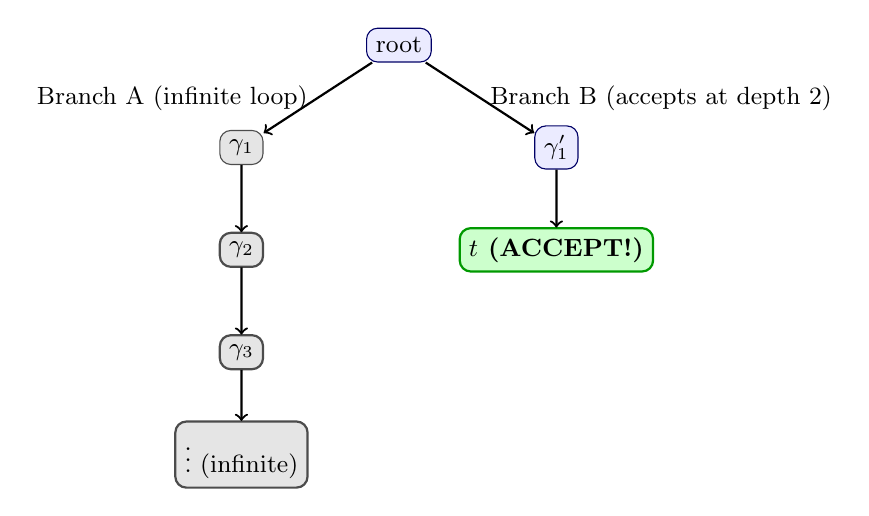
\begin{tikzpicture}[
    level distance=1.3cm,
    sibling distance=4cm,
    edge from parent/.style={draw, ->, thick},
    every node/.style={font=\small},
    acc/.style={fill=green!20, draw=green!60!black, rounded corners,
      font=\small\bfseries},
    inf/.style={fill=gray!20, draw=gray!60!black, rounded corners,
      font=\small},
    cfg/.style={fill=blue!8, draw=blue!40!black, rounded corners,
      font=\small},
  ]
  \node[cfg] {root}
    child {
      node[inf] {$\gamma_1$}
        child {
          node[inf] {$\gamma_2$}
            child {
              node[inf] {$\gamma_3$}
                child {
                  node[inf] {$\vdots$ (infinite)}
                }
            }
        }
      edge from parent node[left] {Branch A (infinite loop)}
    }
    child {
      node[cfg] {$\gamma'_1$}
        child {
          node[acc] {$t$ (ACCEPT!)}
        }
      edge from parent node[right] {Branch B (accepts at depth 2)}
    };
\end{tikzpicture}
\end{center}

\textbf{What DFS does:} It goes down Branch A first. $\gamma_1 \to \gamma_2
\to \gamma_3 \to \gamma_4 \to \ldots$ forever. It \textbf{never comes back} to
try Branch B. The accepting configuration in Branch B at depth 2 is missed.
The DTM loops forever, even though the NTM accepts!

\textbf{What BFS does:}
\begin{itemize}[nosep]
\item Level 0: root. Not accepting. Continue.
\item Level 1: $\{\gamma_1, \gamma'_1\}$. Neither accepting. Continue.
\item Level 2: $\{\gamma_2, t\}$. \textbf{Found $t$!} ACCEPT.
\end{itemize}

BFS finds the accepting config at depth 2. It checks \emph{all} branches at
each depth before going deeper. It can't get ``trapped'' in an infinite branch
because it never goes deeper than level $d$ until it has checked every node at
level $d$.

\textbf{The guarantee:} If there exists an accepting computation of length $k$
(a branch that reaches $t$ in $k$ steps), BFS will find it when it reaches
level $k$. It doesn't matter if other branches are infinite --- BFS processes
level $k$ in finite time (each level has finitely many configurations because
the branching factor is finite).

\kt{BFS is essential because DFS can get trapped in an infinite branch, missing
a short accepting branch. BFS checks ALL branches at depth $d$ before going to
$d+1$, guaranteeing that any finite accepting path is found.}
\end{conceptbox}

\begin{definitionbox}{{Corollaries of the NTM Simulation Theorem}}

The simulation theorem gives us two important equivalences. These are the NTM
versions of the characterizations we already had for DTMs.

\textbf{Corollary 1 (Computably-enumerable languages):}
\fitmath{L \text{ is computably-enumerable} \;\iff\; L = L(N) \text{ for some NTM } N}

\textbf{Plain English:} A language is c.e.\ if and only if some NTM recognizes
it. This is because:
\begin{itemize}[nosep]
\item ($\Leftarrow$): If NTM $N$ recognizes $L$, then by the simulation
  theorem, some DTM $D$ also recognizes $L$. So $L$ is c.e.\ (by the DTM
  definition of c.e.).
\item ($\Rightarrow$): If $L$ is c.e., some DTM recognizes it. Every DTM is
  already an NTM (with $|\delta(q,a)| = 1$ always). So some NTM recognizes $L$.
\end{itemize}

\textbf{Corollary 2 (Computable / decidable languages):}
\fitmath{L \text{ is computable} \;\iff\; L = L(N) \text{ for some halting NTM } N}

\textbf{Plain English:} A language is decidable if and only if some
\emph{halting} NTM decides it. The simulation theorem preserves the halting
property.

\kt{Adding nondeterminism to TMs does not change the classes of c.e.\ or
computable languages. NTMs recognize exactly the same languages as DTMs.
This is the ``same power, different convenience'' story, just like multi-tape.}
\end{definitionbox}